%% Version 4.3.2, 25 August 2014
%
%%%%%%%%%%%%%%%%%%%%%%%%%%%%%%%%%%%%%%%%%%%%%%%%%%%%%%%%%%%%%%%%%%%%%%
% Template.tex --  LaTeX-based template for submissions to the 
% American Meteorological Society[RBR1]
%
% Template developed by Amy Hendrickson, 2013, TeXnology Inc., 
% amyh@texnology.com, http://www.texnology.com
% following earlier work by Brian Papa, American Meteorological Society
%
% Email questions to latex@ametsoc.org.
%
%%%%%%%%%%%%%%%%%%%%%%%%%%%%%%%%%%%%%%%%%%%%%%%%%%%%%%%%%%%%%%%%%%%%%
% PREAMBLE
%%%%%%%%%%%%%%%%%%%%%%%%%%%%%%%%%%%%%%%%%%%%%%%%%%%%%%%%%%%%%%%%%%%%%

%% Start with one of the following:
% DOUBLE-SPACED VERSION FOR SUBMISSION TO THE AMS
% \documentclass{ametsoc}

% TWO-COLUMN JOURNAL PAGE LAYOUT---FOR AUTHOR USE ONLY
\documentclass[twocol]{ametsoc}

%%%%%%%%%%%%%%%%%%%%%%%%%%%%%%%%
%%% To be entered only if twocol option is used

\journal{jcli}

%  Please choose a journal abbreviation to use above from the following list:
% 
%   jamc     (Journal of Applied Meteorology and Climatology)
%   jtech     (Journal of Atmospheric and Oceanic Technology)
%   jhm      (Journal of Hydrometeorology)
%   jpo     (Journal of Physical Oceanography)
%   jas      (Journal of Atmospheric Sciences)	
%   jcli      (Journal of Climate)
%   mwr      (Monthly Weather Review)
%   wcas      (Weather, Climate, and Society)
%   waf       (Weather and Forecasting)
%   bams (Bulletin of the American Meteorological Society)
%   ei    (Earth Interactions)

%%%%%%%%%%%%%%%%%%%%%%%%%%%%%%%%
%Citations should be of the form ``author year''  not ``author, year''
\bibpunct{(}{)}{;}{a}{}{,}

%%%%%%%%%%%%%%%%%%%%%%%%%%%%%%%%%%%%%%%%%%%%%%%%%%%%%%%%%%%%%%%%%%
%% Matt's added packages: (idk if I'm allowed to do this in my submission but I think so)
\usepackage{amsmath}
\usepackage{graphicx}
\usepackage[colorinlistoftodos]{todonotes} %% For comments that will show in the pdf
\usepackage{gensymb} %%for degree symbols mainly



%%%%%%%%%%%%%%%%%%%%%%%%%%%%%%%%

%%% To be entered by author:

%% May use \\ to break lines in title:

%% \title{Trends in Ice Storms throughout the Great Lakes Region}
\title{Recent Changes in Freezing Rain and Ice Storms\\ throughout the Great Lakes Region and Appalachia}

%%% Enter authors' names, as you see in this example:
%%% Use \correspondingauthor{} and \thanks{Current Affiliation:...}
%%% immediately following the appropriate author.
%%%
%%% Note that the \correspondingauthor{} command is NECESSARY.
%%% The \thanks{} commands are OPTIONAL.

    %\authors{Author One\correspondingauthor{Author One, 
    % American Meteorological Society, 
    % 45 Beacon St., Boston, MA 02108.}
% and Author Two\thanks{Current affiliation: American Meteorological Society, 
    % 45 Beacon St., Boston, MA 02108.}}

\authors{Matt Irish\correspondingauthor{Matt Irish, Space Research Building, 2455 Hayward [RBR2]Street, Ann Arbor, MI 48109-2143} and Richard B. Rood}

\affiliation{Department of Climate and Space Sciences and Engineering, University of Michigan, Ann Arbor, Michigan}

\email{mairish@umich.edu}

%% If appropriate, add additional authors, different affiliations:
    %\extraauthor{Extra Author}
    %\extraaffil{Affiliation, City, State/Province, Country}
\extraauthor{William J. Baule\thanks{Current affiliation: MSU address here.}}
\extraaffil{Great Lakes Integrated Science Assessment, Ann Arbor, Michigan.}


%%%%%%%%%%%%%%%%%%%%%%%%%%%%%%%%%%%%%%%%%%%%%%%%%%%%%%%%%%%%%%%%%%%%%
% ABSTRACT[RBR3]
%
% Enter your abstract here
% Abstracts should not exceed 250 words in length!
%
% For BAMS authors only: If your article requires a Capsule Summary, please place the capsule text at the end of your abstract
% and identify it as the capsule. Example: This is the end of the abstract. (Capsule Summary) This is the capsule summary. 

\abstract{Despite the expensive and deadly impacts that freezing rain events have upon major population centers in the Great Lakes region of North America and the region's status as a freezing rain hotspot, little research has been devoted to better understanding the spatial and temporal distribution of these events and their recent trends, especially in regard to anthropogenic climate change. This work extends the most recent Great Lakes freezing rain climatology (1976--1990) to analyze trends and their underlying dynamics by making use of observations made through 2014. To isolate regional trends and determine changes in the synoptic-scale processes driving them, a k-means objective clustering algorithm was used first to create three archetypal synoptic weather patterns associated with freezing rain events and then to group weather stations into regions subject to unique synoptic conditions during freezing rain events. A northward shift in freezing rain frequency is evident across the Great Lakes on an annual basis, along with a modest increase in January and a decrease in March. The intensity of freezing rain events has increased in all regions except South-Central Canada since automated freezing rain instrumentation began in 1995. The largest regional trend has been a **\% decrease (+1.9 hrs/yr/decade) in hourly freezing rain observations in Appalachia since 1976 despite no discernible change in total precipitation. South-Central Canada has seen an increase of **\% (-**hours/decade) in the context of a slight increase in overall precipitation, and the New York City area has seen an increase of  and **\% (-1.3 hrs/yr/decade) despite a trend toward less overall precipitation each year. The low-pressure centers of each of the three synoptic weather patterns have migrated northward on the order of ~100 miles between the first and second half of the 1979--2014 period, consistent with warmer temperatures and northward-moving extratropical cyclones. Observed trends have generally matched or outpaced model projections.}

\begin{document}

%% Necessary!
\maketitle

%%%%%%%%%%%%%%%%%%%%%%%%%%%%%%%%%%%%%%%%%%%%%%%%%%%%%%%%%%%%%%%%%%%%%
% MAIN BODY OF PAPER[RBR4]
%%%%%%%%%%%%%%%%%%%%%%%%%%%%%%%%%%%%%%%%%%%%%%%%%%%%%%%%%%%%%%%%%%%%%
%
\section{Introduction}
The relatively mild temperatures present during ice storms often leave them neglected in discussions of extreme weather events; however, the detrimental impacts of accumulated glaze ice from freezing rain events often compare with those of tornadoes, severe thunderstorms, and in a few severe events, hurricanes. \todo[size=\small]{citations needed} In North America, ice storms occur most frequently in the upper U.S. Midwest, northeastern U.S., southeastern Canada, and in some locations throughout the Pacific Northwest. In the northeastern United States, adjacent to the St. Lawrence river valley, freezing rain was experienced during roughly 5--7 days each year in the middle of the 20th century \citep{changnon2003temporal}. In Pennsylvania, New York, and New England, the probability during a single ice storm glazing of more than 0.64 cm (0.25 inch, the standard used to roughly define the minimum ice accretion constituting an ice storm) during a given year was 88\% \citep{nwsglossary,tattelman1973estimated}. 

Over the past several decades, single storms have caused billions of dollars of damage and taken hundreds of lives[RBR5]. The most obvious impacts of these events are on transportation, but power outages due to heavy icing on power lines are among the greatest challenges. Injuries and deaths from falling trees and power lines are common, and deaths have resulted from carbon monoxide inhalation due to poorly ventilated generators \citep{daley2000outbreak}.  Ice storms can have power generation impacts, with wind turbines forced offline due to blade icing sometimes for days and even up to two weeks in some regions \citep{davis2014forecast}. Data on the costs to generators and ratepayers of such shutdowns have not been analyzed and many system operators do not collect data on wind curtailment. The New England Independent System Operator, the organization responsible for operating that region's power system, reported that shutdowns due to blade icing sometimes account for a substantial portion of the total yearly wind curtailment in the region \citep{bird2014wind}. As development of new wind energy projects accelerates, this makes understanding recent trends in freezing rain occurrence particularly important for financial projections, power system reliability and resilience planning studies, and safety considerations during siting. 

The damage to natural systems by the presence of glaze ice has also been explored, mainly in regard to forest management and damage to vegetation that wildlife relies on for food and shelter \citep{pellikka2000modelling}.

\missingfigure{Will be a cartoon illustration of freezing rain impacts. It's not necessary but I [RBR6]haven't found a good one yet so I thought it might be nice for people to be able to use.}

Ice storms generally occur when the surface temperature is just below freezing. Freezing rain events often form latitudinal bands across the regions they affect, and these bands are expected to shift northward as the climate continues to warm \citep{cheng2011possible,lambert2011simulated}. It is intuitive how this would occur as the 0\degree C isotherm migrates poleward, but this simplistic notion is complicated by the fact that freezing rain events are triggered under several different synoptic conditions and are heavily influenced by both topography and proximity to large bodies of water such as the Great Lakes and the Atlantic Ocean. 

In an effort to understand regional differences in freezing rain formation, \citet{rauber2001synoptic} carried out a manual classification of 411 ice storms occurring east of the Rocky Mountains from 1970-1994 and identified seven archetypal categories of freezing rain storms. These classifications were later consolidated by \citet{erfani2012automated} into three groups by a k-means objective typing algorithm and statistical analysis carried out on the same storms. 

Looking forward into the 21st century, \citet{lambert2011simulated} applied a precipitation typing algorithm to climate model simulations of a moderate warming scenario for 2081-2100 and found that freezing rain events are expected to shift poleward with modest increases in freezing rain incidence to the north and substantial decreases to the south. \citet{cheng2011possible} came to similar conclusions using statistical downscaling and synoptic weather typing of climate projections to predict substantial increases in freezing rain frequency throughout southeastern Canada during the months of January and February (with a progressively greater effect from south to north) and less substantial decreases in the fall and winter months. The two studies, however, focused on slightly different regions and came to differing conclusions about whether seasonal increases overwhelm the decreases on an annually-averaged basis. \todo[inline]{add other freezing rain modeling references here, how winter is changing, limits to modeling unique to fzra and need for obs-based analysis}[RBR7]

%%\subsection{Objective}
\citet{groisman2016recent} provided the first evidence supporting the hypothesis that temporal changes in freezing rain distributions have been observed. Their analysis focused on North America and Europe as a whole and the analysis of trends was limited to concluding that there have been increases in the arctic region of North America and decreases in the southeastern U.S. Most ice storms and the greatest impacts on humans, however, are concentrated between those two extremes, in the mid-latitudes.

The most recent freezing rain climatology to focus on the Great Lakes region was published in 2000, made use of observations from 1976 to 1990 \citep{cortinas2000climatology}, and did not analyze trends. The purpose of this paper is to build upon that climatology by analyzing trends in the frequency, intensity, and duration of freezing rain events through 2014 and then to identify the underlying changes in the weather systems that bring them about. These changes in climate dynamics are compared with those previously linked to human emissions of greenhouse gases in the scientific literature to investigate how the observed trends fit into the larger frame of anthropogenic climate change.

Need a paragraph defining what is to come and the basic steps of the analysis.  Regional and synoptic classifications.[BJB1]


\section{Data}
The study area was defined similar to that of \citet{cortinas2000climatology}, but reaching further eastward, from 105\degree W to 60\degree W and 25\degree N to 60\degree N. It spans the U.S. states of Illinois, Indiana, Iowa, Michigan, Minnesota, New York, Ohio, Pennsylvania, and Wisconsin, as well as the Canadian provinces of Ontario and Quebec (Fig. \ref{fig:trendmap}).

The infrequent nature of freezing rain events suggests a signal-to-noise ratio close to one, and the use of weather station observations for trend analysis is made difficult by instrumentation changes in the observational record and the highly localized nature of freezing rain formation.  The observation of freezing rain uses the hourly surface observations from the Automated Surface Observing System (ASOS), provided as part of the Integrated Surface Database maintained by the National Centers for Environmental Data \citep{smith2011integrated}. The observations span from 1976 to 2014. [BJB2]

\todo[size=\small]{BJ stuff}After filtering the ASOS data to eliminate special observations and objectively normalize the number of observations down to one per hour, the time series of observations were almost complete for most stations.  A standard of 90\% was adopted for this work, compared with \citet{cortinas2000climatology}, which excluded any location with less than 80\% present weather reports. Some locations were excluded for which manual observers were not present during the night throughout the winter months in the mid-1990s and earlier. Despite efforts in quality control, issues remain with intermittent manual observation during some hours in the first two decades of observations. After performing this quality control, 97 stations out of an initial 121 met the criteria to be used in the analysis, and an average of 97.4\% of hours each year were accounted for at the included stations.[RBR8]

An important caveat regarding the use of the ASOS dataset is that it spans a transition in observing techniques from a period involving strictly manual freezing rain observations (1976--1994) to the automation of reporting with new freezing rain instruments beginning in 1995 \citep{ramsay1995status,asos1998}. Comparison of pre- and post-transition freezing rain frequencies show that any bias present does not appear to overwhelm any temporal or spatial trends.[RBR9]

Given the value of analyzing freezing rain based on synoptic weather conditions, synoptic-scale weather variables were examined using the North American Regional Reanalysis (NARR) produced at the National Centers for Environmental Prediction \citep{mesinger2006north}. The variables of interest were mean surface level (MSL) pressure, 850 mb geopotential heights, and air temperature at 2 m. The NARR was chosen for its consistency of temporal assimilation, assimilation of precipitation data, and high resolution (32 km at 3-hour intervals). The reanalysis begins in 1979, leaving 1976-1978 ASOS observations outside the range that can be investigated[RBR10].


\section{Methods}
A straightforward trend analysis only requires the total number of hours of freezing rain recorded over a time interval. However, to gain a fuller picture of how and why such events may have changed, more definition of a freezing rain event, or ice storm, is necessary. The U.S. National Weather Service terms an ice storm an occasion "when damaging accumulations of ice are expected during freezing rain situations," adding that the term generally refers to accumulations of 0.64 cm (0.25 in.) and greater \citep{nwsglossary}. Although ice storms are the topic of interest in this work, such a criterion is inappropriate for this analysis since ice accretion occurs at different rates on different surfaces and under different conditions, and is poorly estimated using variables such as wind and dewpoint temperature. 

Therefore, rather than an ice storm, a freezing rain event is used in this analysis. A freezing rain event is defined as having begun at the first hourly report of freezing rain anywhere in the region and continuing until at least three hours has elapsed without any further reports of freezing rain across the domain of study. For purposes of classifying freezing rain events, events with less than four reports of freezing rain were excluded to eliminate hyper-localized reports; however, all observations of freezing rain are included in the initial frequency trend analysis. Our results were somewhat sensitive to the choice of hours defining an event when the number of minimum reports was less than four and the number of intervening no-report hours was more than three. The synoptic weather typing was most sensitive, with noisy synoptic weather conditions likely being introduced by localized and short-lived events. A further analysis of these events showed that they make up only **\% of all observations[RBR11].

\subsection{Analysis of trends}
A mix of parametric and non-parametric methods were used in the trend analysis depending on the parameter being studied. Changes in the intensity of freezing rain were analyzed using standard least-squares linear regression. The existence of trends in the seasonal and annual frequency of freezing rain reports was tested for using a modified form of the non-parametric seasonal Mann-Kendall test for a monotonic trend and the Theil-Sen method for calculating a linear slope. Both are techniques to assess monotonic trends \citep{chandler2011statistical}. Though they offer less statistical power than parametric methods, such tests were chosen because the time series of freezing rain reports are positively skewed[RBR12]. This is intuitive, since freezing rain reports are rare, discrete events with some "non-detect" periods (time intervals for which there were zero freezing rain observations), and was confirmed by plotting histograms of the observations.

\subsubsection{Modified seasonal Mann-Kendall test for monotonic trend}
The Mann-Kendall test assesses the relative magnitude (rank) of observations rather than their absolute values. The null hypothesis of the test is that the data are randomly ordered as opposed to exhibiting a monotonic trend in time. The test is carried out for the sequence of both annual and monthly total freezing rain reports at each location[RBR13], $y_1,\ldots,y_T$. The differences of each permutation of pairs $\{d(t_1,t_2)=y_{t2}-y_{t1}:t_2>t_1\}$ is calculated for all $T$ observations and then assigned values of $+1$ for positive differences, zero for ties, and $-1$ for negative differences. The test statistic for the original Mann-Kendall method, $S$, is the sum of all these values:

\[\sum_{t_1=1}^{T-1}\sum_{t_2=t_1=1}^T\text{sgn}[d(t_1,t_2)],\] where\\
\[\text{sgn}[d(t_1,t_2)]=\begin{cases} 1 & \text{if } d(t_1,t_2)>0\\ 0 & \text{if } d(t_1,t_2)=0\\ -1 & \text{if } d(t_1,t_2)<0.\\ \end{cases}\]

So $S$ can take any integer value from $-T(T-1)/2$ to $T(T-1)/2$. $S$ is proportional to the nonparametric Kendall's rank correlation coefficient, $\tau$, a measure of the rank correlation between the annual or monthly freezing rain reports and time with range $\tau=\pm1$:

\[\tau=\frac{2S}{T(T-1)}\]

If $S\approx0$, then $\tau\approx0$ and the null hypothesis of no trend is accepted, whereas if  $S\approx\pm T(T-1)/2$, $\tau\approx\pm1$ and the null hypothesis is rejected. 

The test described above is expanded into the multivariate "seasonal" [RBR14]Mann-Kendall trend test to explore monthly trends and to accommodate serial dependence [RBR15]within the dataset. This involves expanding the time series into a $T\text{ by }p$ matrix, where the number of seasons $p=12$ (meaning that the term "seasonal" in this application is referring to months rather than the four seasons of spring, summer, autumn, and winter). The null hypothesis is that for each of the $p$ seasons, the $T$ observations are randomly ordered. The calculation of the new test statistic and its variance is too involved to fully describe here,[RBR16] but \citet{hirsch1984nonparametric} (pg. 728) detail the derivation, which focuses on summing contributions from individual seasons.

The original Mann-Kendall test and its monthly expansion assume the time series is serially independent, in which case the null distribution can be approximated by a normal distribution with mean zero and an analytically-defined variance \citep{kendall1955rank}. But this is not the case for some of the freezing rain time series analyzed here, so the test had to be modified with a different variance. This is akin to considering the degrees of freedom in parametric significance tests. Serial dependence in the dataset was tested for by calculating the autocorrelation coefficient (defined here as the non-parametric Spearman correlation coefficient for a time lag of one year) at each location. The median autocorrelation across the 97 ASOS stations was a fairly small $r_s = 0.0406$.  There were, however, several stations with statistically significant ($p<0.05$) autocorrelations as high as $r_s = 0.5291$. The required modification to the monthly Mann-Kendall test further reduces statistical power as compared with parametric methods, but was considered necessary to maintain statistical rigor. The modified variance calculation was implemented in MATLAB according to the method described by \citet{hirsch1984nonparametric}. [BJB3]

\subsubsection{Theil-Sen slope estimator}
In the case that the Mann-Kendall test indicates a monotonic trend exists, the trend is assumed to be linear and the slope calculated. The Theil-Sen slope estimator is a method commonly paired with Mann-Kendall; it is much more accurate than simple linear regression for non-normal data and is robust in the presence of outliers. The slope is defined as the median of the slopes calculated between every permutation of points in the time series, $\{d(t_1,t_2)/[t_2-t_1]:t_2>t_1\}$. As a linear slope estimation, it can be seen as the "typical" index of change over a unit of time \citep{chandler2011statistical}. The confidence interval is then calculated by computing an inverse normal cumulative density function[RBR17].

\subsection{Classification of regions and analysis of trends in meteorological forcing}
An initial inspection of the temporal and spatial evolution of freezing rain---diurnally, monthly and annually as well as across the domain and at a higher, regional resolution---was carried out to look for clues regarding changes in physical mechanisms.  This is difficult because of the rare and highly local nature of the events---often just a few large storms every year or so obfuscate any slower underlying changes.

As mentioned in the introduction, synoptic conditions during ice storms can be broadly categorized into several distinct archetypal patterns, varying from those caused by extratropical cyclone-anticyclone interactions (mainly in the Midwest to southeastern Canada) to those caused mainly by topography (cold air damming and trapping throughout the Appalachian[RBR18] Range and along its eastern slopes). By analyzing these synoptic conditions and then classifying ASOS stations into regional groups that share similar conditions and freezing rain frequency distributions, we identify regional similarities in the dynamics driving freezing rain events. The goal is to link the events to weather-scale processes, and then, to models' abilities to represent those processes.

A synoptic weather typing and clustering procedure is carried out as follows:
\begin{enumerate}
\item
For each of 1211 events identified across the study region from 1976 to 2014, two 105x99-[RBR19]grid-cell anomaly maps were obtained--one of MSL pressure and one of 850 mb geopotential height--[RBR20]from the three-hourly NARR output closest to the middle of event occurrence. Anomalies were determined by subtracting the monthly climatology of the entire 1979--2014 period. 
\item
The k-means clustering algorithm (with $k=3$, in accordance with \citet{erfani2012automated} and verified using silhouette plots) was applied to the anomaly maps and the resulting centroid maps were constructed. These centroid maps represent the mean pressure anomalies for each of the three storm patterns.
\begin{itemize}
\item
Anomaly maps were reshaped into vectors and the vectors for MSL pressure and 850 mb[RBR21] heights were concatenated, creating a matrix with each row representing an event and each column representing a spatial grid cell. k-means clustering was chosen since it performed the best in \citet{erfani2012automated}'s freezing rain synoptic typing validation, outperforming hierarchical and average linkage methods.
\item
Events were classified into one of three clusters and three centroid maps of MSL pressure anomaly and 850 mb height anomaly were created and analyzed.
\item
The clusters were compared to the archetypal patterns manually classified by \citet{rauber2001synoptic} for physical intuition.
\end{itemize}
\item
The k-means clustering algorithm (with $k=5$, selected by analyzing silhouette plots) was applied again to group stations into five regions by clustering based on the total number of observations of freezing rain attributed to each of the three synoptic types at each station.
\begin{itemize}
\item
A sixth region was manually created by separating four stations in the New York City-Long Island area from another cluster due to the indication that they experience maritime influences that were not well-represented in the clustering. This is consistent with prior work by \citet{bernstein2000regional} establishing the importance of proximity to bodies of water in determining local freezing rain occurrence. The stations manually assigned to the region are located in the Humid Subtropical Koppen climate zone, whereas all stations further inland in New York State are in humid continental [RBR22]zones.
\item
The regions are compared in terms of the prevalence of storms of each of the three types.
\item
Trends are analyzed by region. (I think I removed this.)
\end{itemize}
\end{enumerate}

To link freezing rain trends with possible changes in the meteorological forcing of events, steps 1 and 2 were repeated, dividing the time record into two spans.   The first observation span, 1979--1996 contained 586 events.   The second observation span, 1997--2014 had 625 events.  The new centroid maps are compared to old ones to identify any changes in synoptic types. In addition to rerunning the k-means algorithm to create new clusters, the events in the more recent 1997--2014 period were also classified into the original clusters created from the 1979--2014 dataset by assigning each one according to the minimum Euclidean distance between the event and the centroids. 

Producing separate cluster results for each of the two periods allowed analysis of how underlying modes themselves may have changed, and binning the more recent events to the original clusters trained on the first period made it possible to investigate how the relative importance of different archetypal patterns may have shifted.

\section{Results}

\subsection{Observed trends at individual stations and domain-wide}

\todo[inline]{ADD: (-1.5$\pm$2.1\degree C [1$\sigma$] in the Great Lakes and Northeast during an event)}

Figure \ref{fig:trendmap} depicts linear trends in total annual hours of freezing rain as calculated using the Theil-Sen method at all 97 ASOS stations. The values are shown as percentage change from a 1976--1985 baseline to the 2014 total hours of freezing rain expected by the trend line. As shown, the modified Mann-Kendall test indicated the existence of monotonic annual trends at only 10 locations at the $p=0.05$ significance level. While there appears to be a general decrease in annual hours of freezing rain in the south of the region and an increase to the north in south-central Canada, much of the mid-latitudes has not experienced a consistent trend over the past 39 years. This is somewhat intuitive, since expected decreases in the "shoulder" fall and spring months and increases during the mid-winter months may be expected to have competing effects on the overall annual freezing rain frequency.

\begin{figure*}
\centering
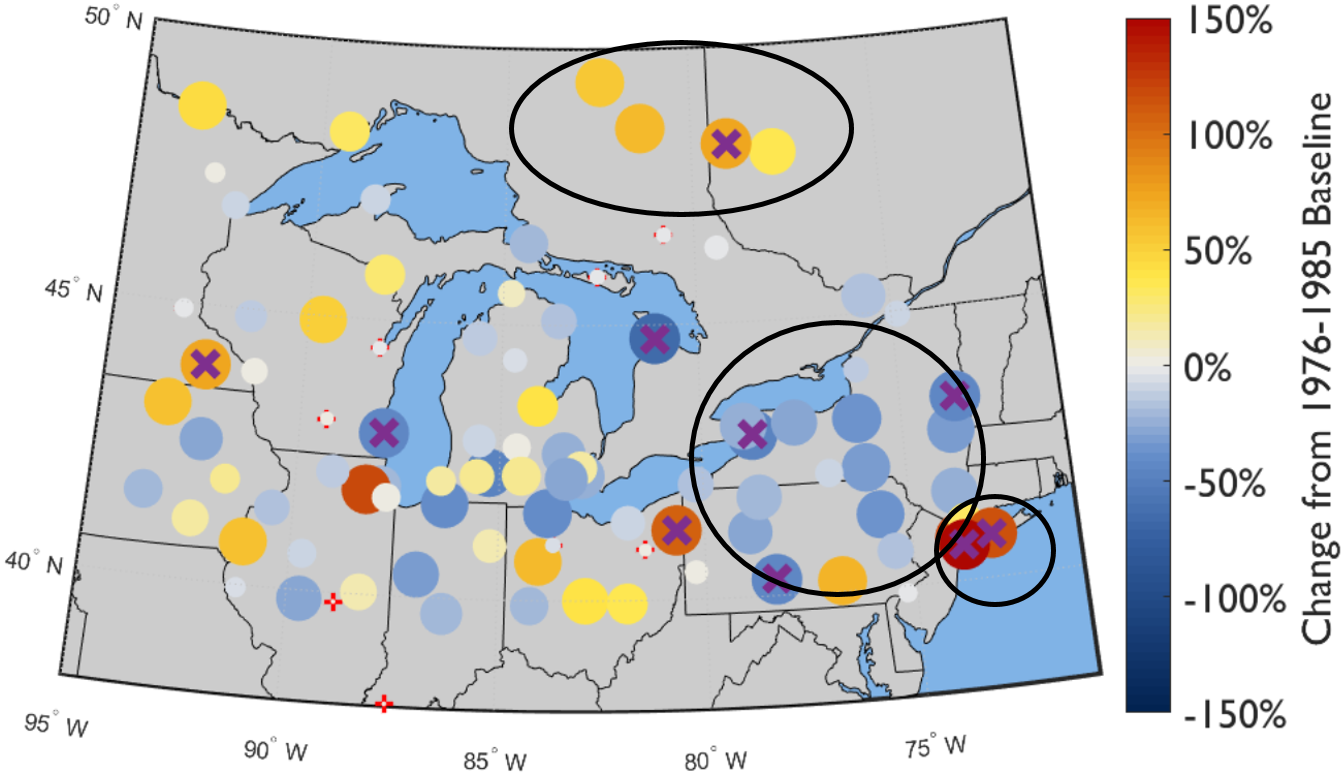
\includegraphics[width=1.0\textwidth]{trendmap.png}
\caption{\label{fig:trendmap}Map of the region of interest showing trends in total annual number of hours of freezing rain reported computed using Theil-Sen method. Locations are scaled by confidence level ($1 - p$) [with plus signs denoting stations with small circles, for clarity]. Xs denote locations where modified Mann-Kendall test indicates a monotonic trend at the $p<0.05$ level. Note: baseline is first decade of observations.}
\end{figure*}
\todo[size=\small]{re: figure: get rid of black circles. Add baseline map + map showing abs trends in hours.} 

Initial inspection of the spatial variation in Figure \ref{fig:trendmap} highlights the need for the definition of regions and a description of their trends, to be discussed in the next sections. Stations along the Appalachian Mountains, for example[RBR23], which frequently experience topography-forced events, have experienced a consistent decrease in freezing rain event frequency, whereas stations centered on Long Island[RBR24] indicate substantial increases.  

\begin{figure*}
\centering
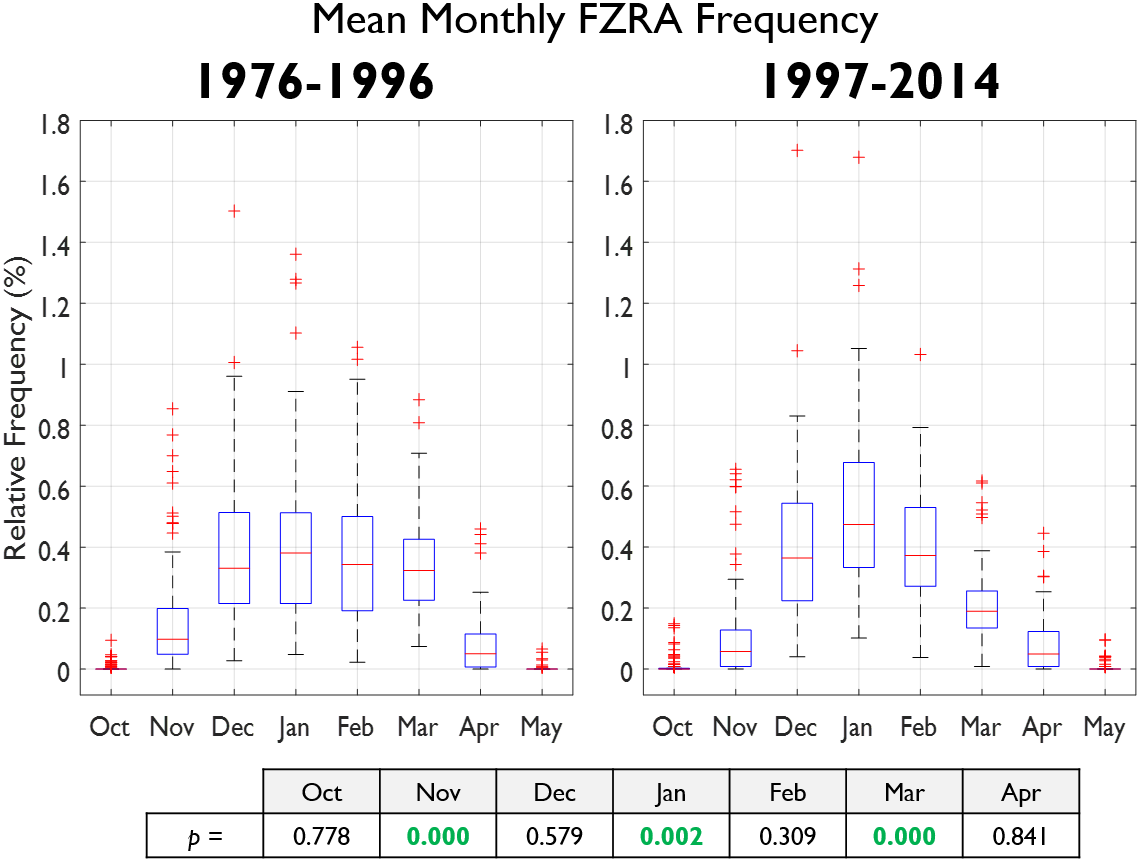
\includegraphics[width=.9\textwidth]{Seasonal.PNG}
\caption{\label{fig:seasonal} Comparison of seasonal frequency of freezing rain events between the first 21 years in the study period and the last 18 (to better coincide with the NARR-based dynamics analysis below). Red lines demarcate mean values, boxes signify 25-75\% percentiles, whiskers inner fences, and red plus signs indicate outliers. Table lists $p$-values calculated using Mann-Whitney rank sum method to test for difference in median value.}
\end{figure*}
\todo[size=\small]{re: figure: add Mann-Whitney p-values in their own row.}

Monthly trends in freezing rain frequency estimated using the modified seasonal Mann-Kendall test reveal a domain(?)-wide significant monotonic trend only for March. (not shown, correct?) A weaker hypothesis is that the average freezing rain frequency for some months has changed.[RBR25] This was tested for using the Mann-Whitney test, a non-parametric counterpart to the two-sample t-test that determines whether the medians of two series are different from one another. Figure \ref{fig:seasonal} shows the frequency … and the $p$-values calculated for each month after computing the Mann-Whitney test, which independently compares the rank of all entries of the two time series for the 1976--1996 period and the 1997--2014 period. As shown, the median duration of freezing rain in the months of November and March has changed, along with the mid-winter month of January. The box-and-whisker plots show the "tightening up" of the winter distribution of freezing rain occurrence, as suggested by prior studies like \citet{cheng2011possible}, has likely begun to occur. However, all that can be said to be robust from this analysis of seasonality is that the median freezing rain frequency has changed in recent years for the months of November, January, and March, and that there has been a robust region-wide decrease in freezing rain occurrence during March. (This is really like a shortening of winter to a 1 month season!)

\begin{figure*}
\centering
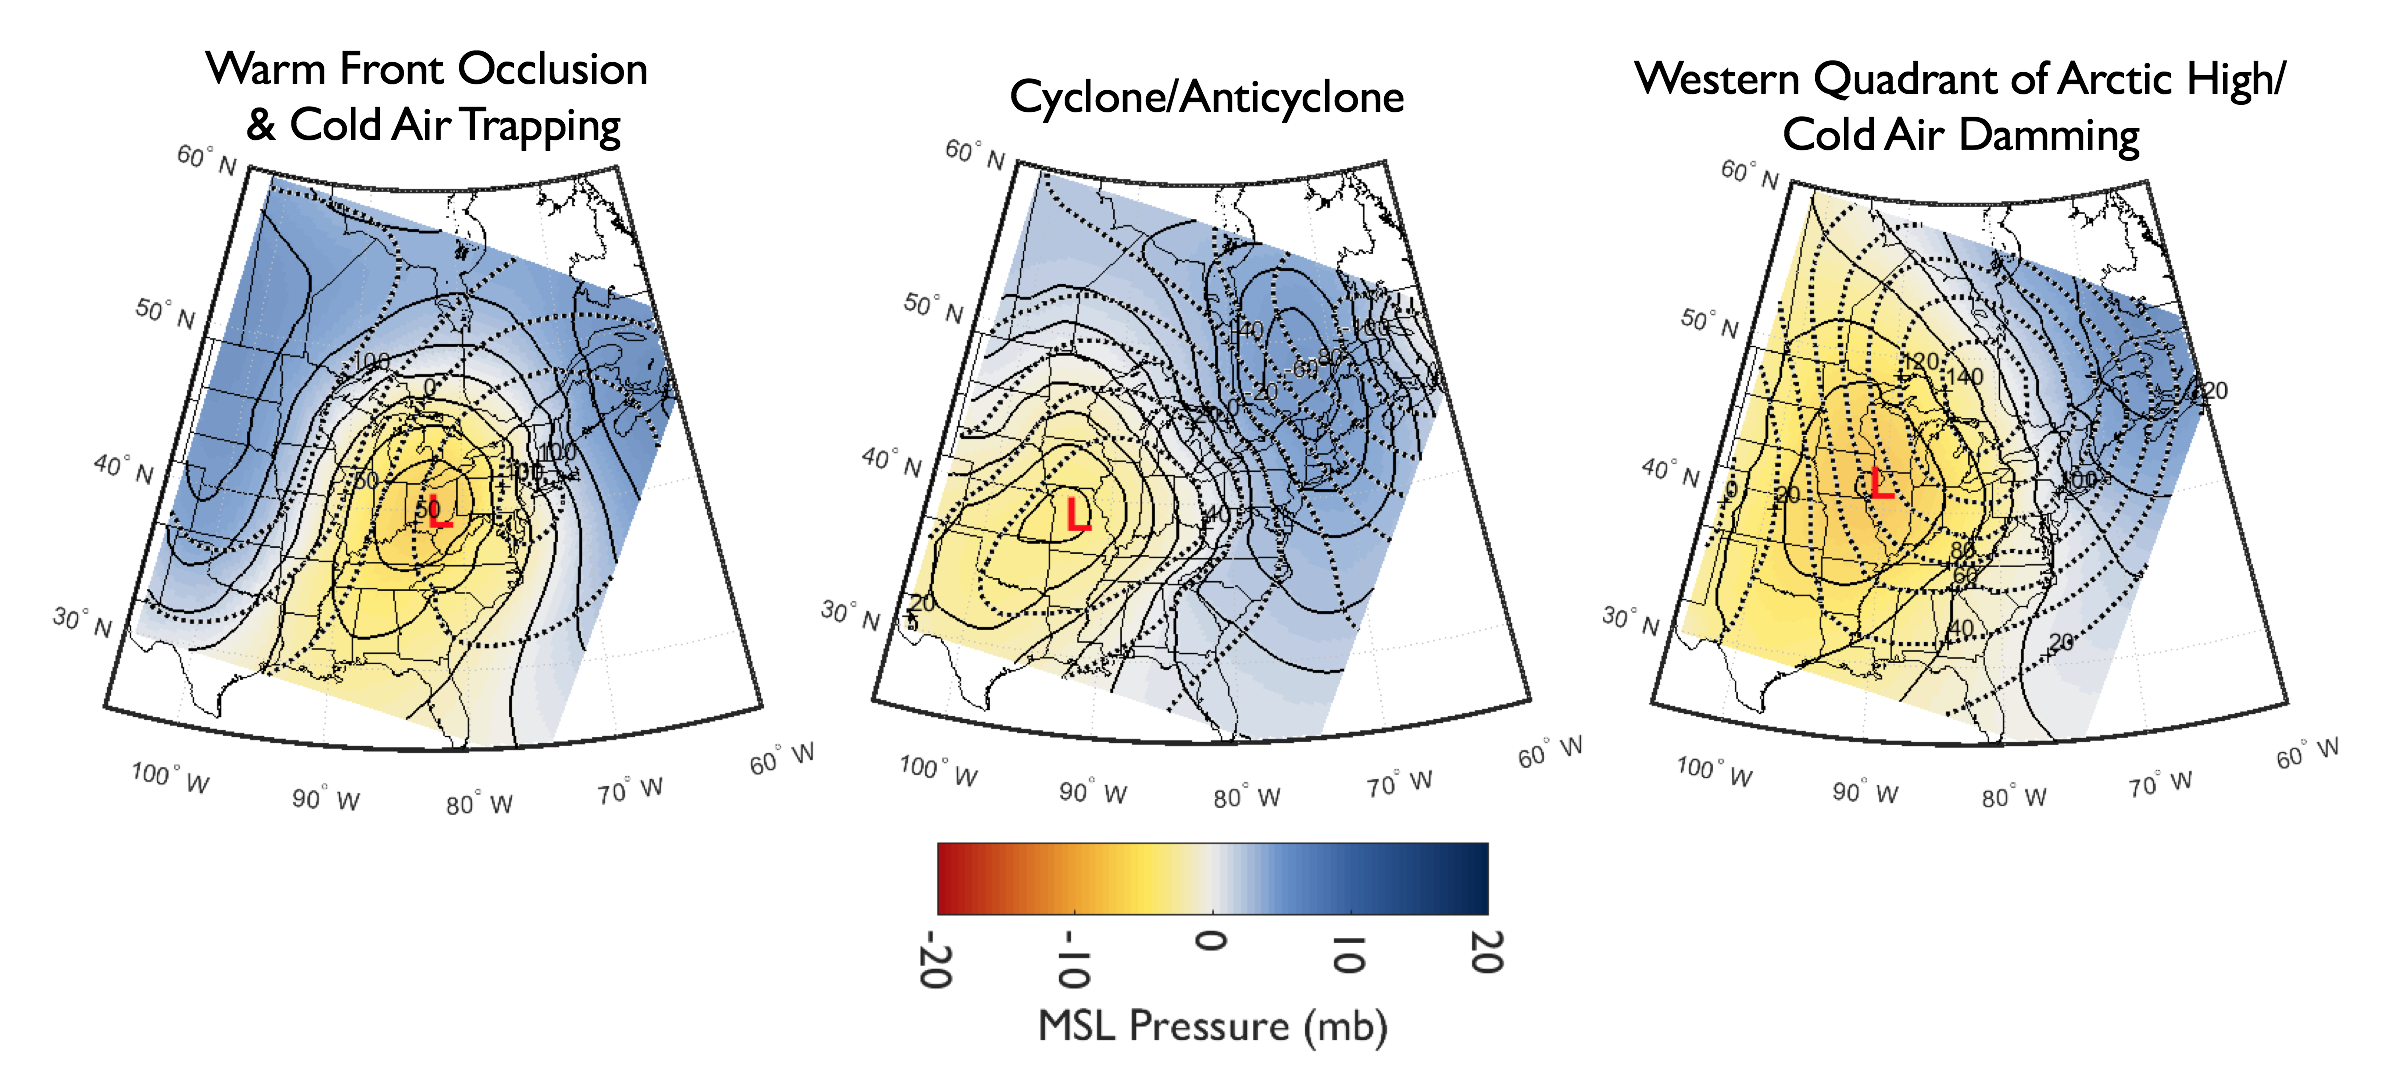
\includegraphics[width=1\textwidth]{Cluster_Centroids.png}
\caption{\label{fig:centroids} Centroid maps of cluster analysis  used to create three archetypal storm patterns. Solid lines refer to MSL pressure anomalies and dotted lines demarcate 850 mb geopotential height anomalies. Color bar shows anomalies, not absolute pressures.}
\end{figure*}
\todo[size=\small]{re: figure: add 0 deg isotherms. Also maybe make maps bigger?}

\subsection{Classification and analysis of regions}
\subsubsection{Clustering of storms into three archetypal patterns}
The k-means clustering algorithm used to group storms into three archetypal patterns resulted in the centroid pressure and geopotential height anomaly maps shown in Figure \ref{fig:centroids}. \citet{erfani2012automated} produced average anomaly maps of Rauber's manually selected groups that were used here for comparison. Table \ref{archetypalpatterns} summarizes these comparisons and key statistics for each cluster \todo[size=\small]{add zero deg isotherm to each map} [RBR26].

The first cluster (Figure \ref{fig:centroids}, left) is similar to Rauber's pattern B, describing freezing rain events that occur at the occlusion sector of warm fronts, as well as Rauber's pattern G, describing cold air trapping. The former occurs just north of the 0\degree C surface isotherm when warm air overruns a subfreezing surface layer. Cold air trapping occurs when approaching continental cyclones advect warm air over the Appalachians, trapping cold air in valleys at the surface and leading to freezing rain. Both MSL pressure and 850 mb anomalies closely resemble those plotted by \citet{rauber2001synoptic}, where  8.1\% of freezing rain events between 1970-1994 were classified as being caused by these conditions. \todo[size=\small]{compare with \% from this study}

The second cluster (Figure \ref{fig:centroids}, center) represents the extratropical cyclone-forced storm that most often affects the Midwestern U.S. and especially its southern region (Rauber pattern C). Storms that take on this pattern were identified by Rauber to be some of the longest in duration and most damaging throughout the Midwestern U.S., due to their high-pressure gradients and the higher winds that result. \todo[size=\small]{compare with \% from this study}

The third cluster (Figure \ref{fig:centroids}, right) is similar to Rauber's patterns D and E. The D group refers to systems that produce freezing rain in the western quadrant of arctic high-pressure anomalies interacting with warmer air from the Southeast. The E pattern describes cold air damming, synoptic conditions which trigger freezing rain when arctic air masses are dammed against the eastern slopes of the Appalachian range and warmer air moving in as a result of easterly flow from the Atlantic overtakes it. Rauber identified this archetypal pattern as contributing to 5.7\% of all storms and many of the longest, with a quarter of events lasting longer than 12 hours.\todo[size=\small]{compare with \% from this study} Freezing rain from these systems would be expected in southern Quebec and Ontario, in the freezing rain hotspots of Ottawa and Montreal and throughout Appalachia.[RBR27] 

\begin{table*}
\label{archetypalpatterns}
\caption{Archetypal patterns of synoptic conditions during freezing rain events as determined through k-means clustering.}
\begin{tabular}{p{0.05\linewidth}p{0.3\linewidth}p{0.1\linewidth}p{0.1\linewidth}p{0.1\linewidth}p{0.1\linewidth}p{0.05\linewidth}}
\topline
Cluster & Description                 & Similar to Rauber patterns & No. of events & Mean duration (hrs.) & \% of reports "light" intensity &  \\ 
\midline
1       & Warm front occlusion and cold air trapping       & B and G      &           &                                          &                                                     &  \\
2       & Cyclone/Anticyclone                              & C            &           &                                          &                                                     &  \\
3       & Western quadrant of arctic high/cold air damming & D and E      &           &                                          &                                                     &  \\
\botline
\end{tabular}
\end{table*}


\subsubsection{Clustering of stations into regions}
Carrying out the second clustering analysis, this time using the number of storms of each pattern recorded over the entire 1979--2014 period at each station, the stations were aggregated into five regions. These regions are referred to according to their geographical location. Though the four stations in the New York City and Long Island area were included in the South Central group by the algorithm, these were manually separated into a separate group based upon their markedly different trends in frequency (see Figure \ref{fig:trendmap}). 

Figure \ref{fig:regional_breakdown} depicts the six regions. Using trial and error along with a silhouette plot to determine the ideal number of clusters, several stations (including the four reclassified into a NYC region) were determined to be close to a boundary between two clusters and were sometimes grouped differently depending on the initial conditions of the clustering algorithm. Several other stations that were near boundaries could have been manually reclassified, but most of those were geographically close to the boundaries with different regions, so no further reclassifications were made. 

\begin{figure*}
\centering
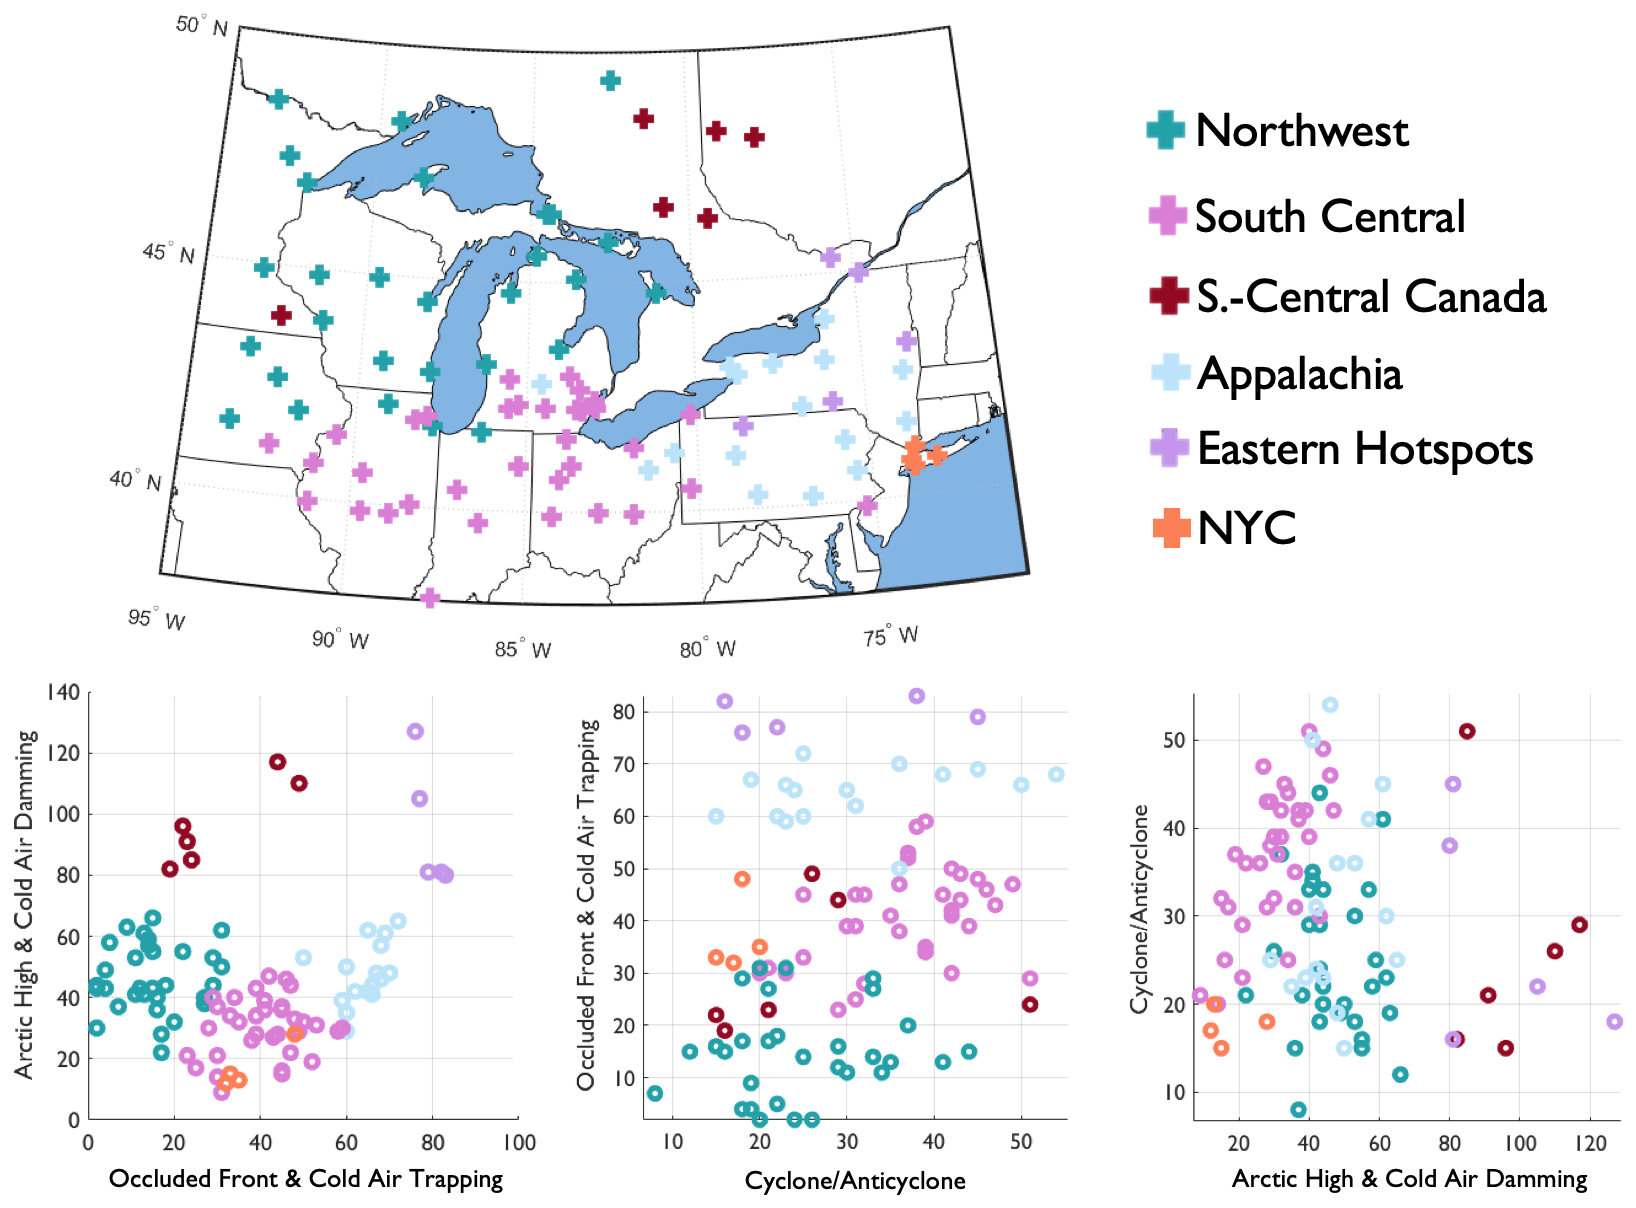
\includegraphics[width=1\textwidth]{regional_Breakdown.png}
\caption{\label{fig:regional_breakdown} Seven regions determined using k-means clustering to group stations with similar freezing rain profiles (top). Prevalence of total events in each of the three ice storm patterns by station and region (bottom). Axes refer to the total number of storms recorded for that pattern in the 1979--2014 period and points in the scatter plots represent stations.}
\end{figure*}

It is important to highlight that no geographic information was introduced directly into the clustering algorithm, so ASOS stations that are nearby one another being grouped into one contiguous cluster indicates a correlation in terms of the meteorological conditions that give rise to ice storms in those areas. The several stations that appear as physical outliers (e.g. the station at Rochester, Minnesota that is classified into the S.-Central Canada region) were not near the boundaries of their clusters, and as such were not reclassified. Overall, the regions agree with physical intuition regarding the meteorological forcing behind freezing rain events. 

A visual analysis of the regional clusters is shown in Figure \ref{fig:regional_breakdown}. Regional distributions of event totals largely adhere to what was expected in the discussion of the three synoptic patterns above. The leftmost plot, comparing the prevalence of events forced by the western quadrant of arctic highs/cold air damming and the occluded sector of warm fronts/cold air trapping shows the most variance between stations and looks somewhat similar to the geographic distribution of stations. Only stations throughout Appalachia [RBR1]have received upward of 60 ice storms attributable to the topographical effects of cold air trapping and/or being located in the northeastern region of occlusion zones, while the S.-Central Canada region has experienced as little freezing rain due to the occluded front/cold air trapping pattern as other region but shows enhanced influence of the arctic high/cold air damming pattern. The second plot shows that the influence of the anticyclone-cyclone interaction is spread fairly evenly across the different regions. The third plot highlights the lack of influence exerted by the west quadrant of arctic highs/cold air damming pattern on freezing rain occurrence throughout the Midwestern U.S. The NYC region observes the least freezing rain on average, with most of it being attributable to the occluded front/cold air trapping pattern. Despite showing different overall trends, the NYC region stations could be grouped into either of the Midwestern U.S. categories but would not likely have become their own category. This highlights the limitations of this objective typing method[RBR2].
 

\subsection{Changes in meteorological forcing}
Changes in meteorological forcing were investigated by separately clustering the first and second half of the 36-year time period of NARR coverage and examining the changes in centroid anomaly maps from the former to the  latter half of observations. While there are close similarities between the clusters identified in the analysis of regions above, several notable differences are observed for the clusters as computed for the two separate time periods and for the clusters as trained upon the first half of the time period later in this section. As such, the clusters are numbered to highlight that distinction.

The results of the k-means clustering algorithm are depicted in Figure \ref{fig:clusters}. \citet{erfani2012automated} found that three clusters were appropriate to describe the significantly different archetypal patterns causing freezing rain by analyzing wind and precipitation variances for different values of $k$. Their analysis, however, carried out two different clustering algorithms, one for MSL pressure and one for pressure aloft, whereas here both are considered in the same clustering process. 

Comparing with the archetypal patterns set out by Rauber and the clusters identified by Erfani, Cluster 1 indicates a cyclone/anticyclone setup (Rauber pattern C). The northward shift and apparent intensification of the cyclone is striking. This is consistent with observations dating back to roughly 2000 of a northward shift in cyclone tracks, thought to be forced at least in part by increasing temperatures due to enhanced mixing ratios of atmospheric CO$_2$ \citep{mccabe2001trends}. While becoming less frequent, these cyclones have also become more intense. These historically have also been the longest-lasting events, with 25\% of these events lasting more than 24 hours \citep{rauber2001synoptic}. 

Little change seems to be observed in Clusters 2 and 3 across the two periods. Cluster 2 encapsulates Rauber patterns F and G, the topography-forced cold-air damming and trapping conditions. A similar cluster was created by Erfani. Cluster 3, which is similar to Rauber's pattern B, characterizing the classical formation of freezing rain caused at the warm front and occlusion sector of cyclones, appears to have changed little as well.\todo[size=\small]{take a closer look. There are some clear changes, esp. with northward movement of L pressure center in 2 and an eastward push of the low pressure system in 3}

\begin{figure*}
\centering
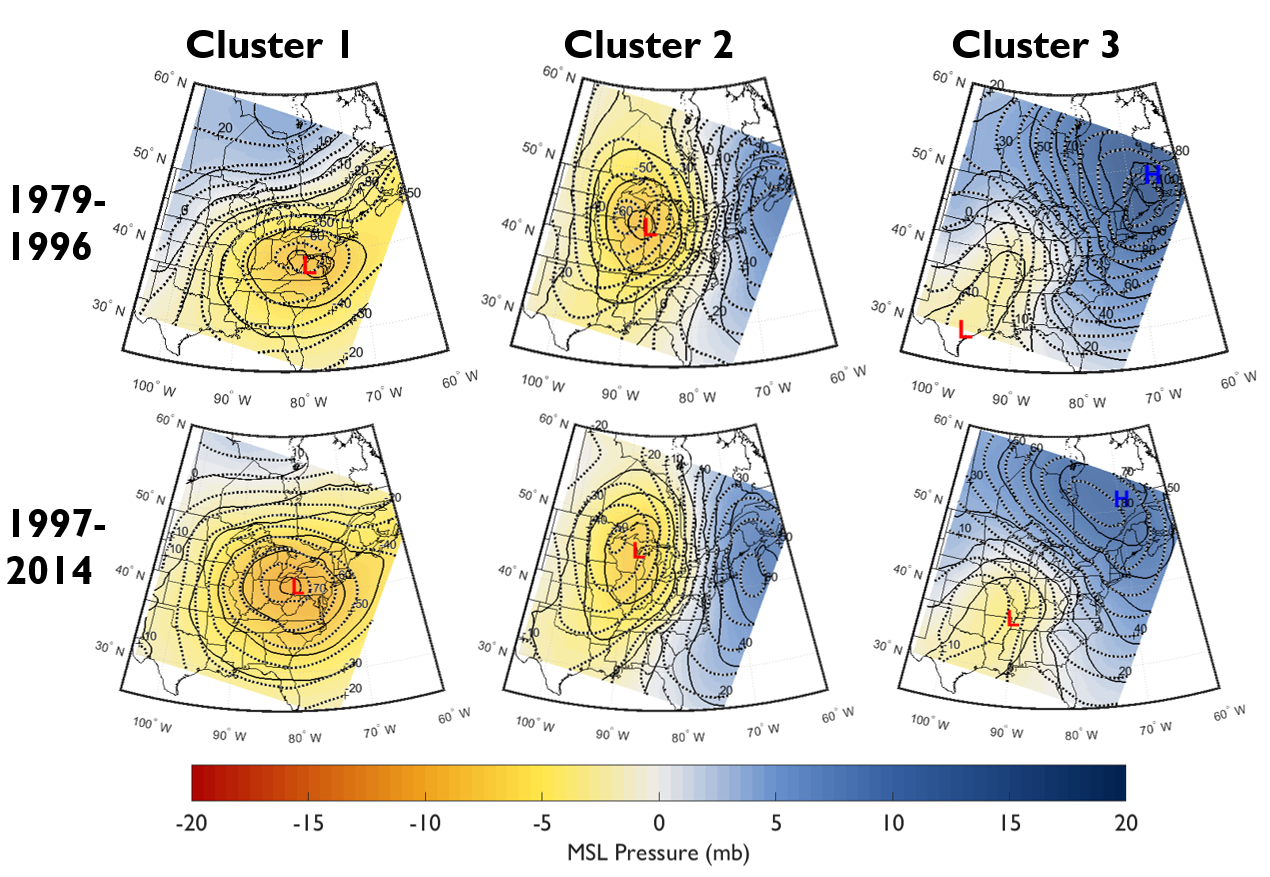
\includegraphics[width=\textwidth]{Clusters.PNG}
\caption{\label{fig:clusters} Freezing rain event archetypal patterns created using k-means algorithm with $k=3$. Color ramp and solid lines refer to MSL pressure anomalies in mb, while labeled dotted lines refer to 850 mb geopotential height anomalies in m.}
\end{figure*}

\begin{figure}
\centering
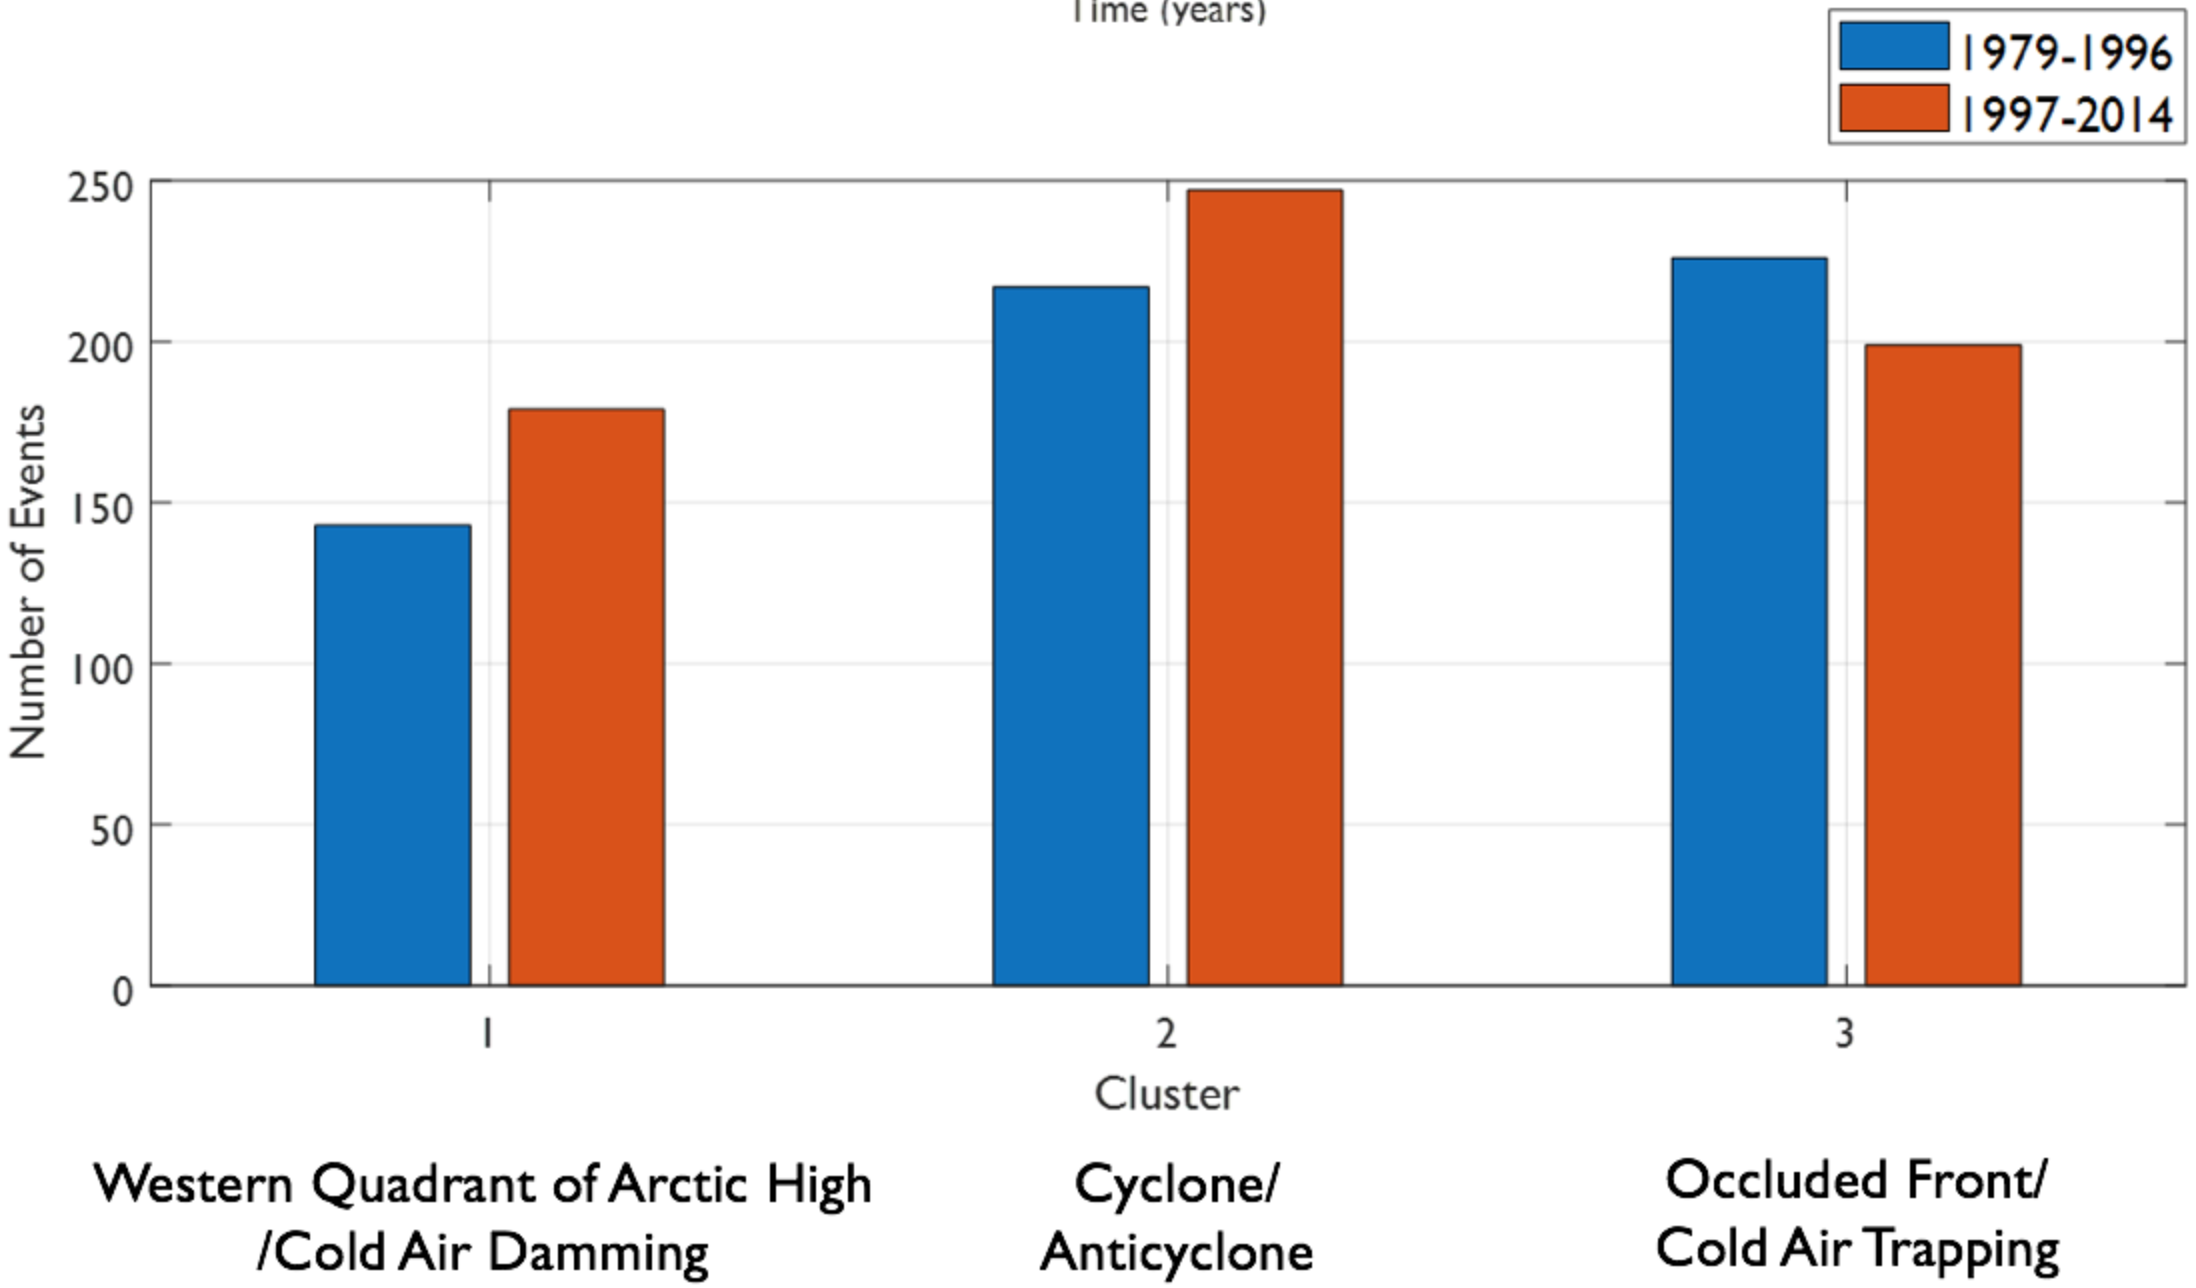
\includegraphics[width=0.5\textwidth]{Storm_Pattern_Change.png}
\caption{\label{fig:clusterchange} Timeline showing all events as classified into each of three clusters as calculated for the 1979--1996 period (top) and change in classification of events from the 1979--1996 period to the 1997--2014 period where the latter period is classified according to the centroids trained on the earlier period (bottom).}
\end{figure}

To investigate any changes in the relative contribution of each archetypal pattern to annual freezing rain totals, the prevalence of events in the 1979--1996 period is compared with that of events from the 1997--2014 period after each event has been assigned to a centroid computed from the earlier data. Figure \ref{fig:clusterchange} is a bar graph showing the changes in the number of freezing rain events associated with each pattern. 586 events were identified during the first 18-year period, and 625 events were identified during the second period, an overall increase of 6.6\%. The number of freezing rain events under Clusters 1 and 2 \todo[size=\small]{Get consistent with either naming clusters by numbers or not} rose substantially, indicating an interdecadal increase in the number of the often lengthy extratropical cyclone/anticyclone-forced events (25.2\%) as well as those forced by topography in Appalachia and eastward (13.8\%). The number of storms caused in the classic warm front/occlusion zone setup decreased 13.6\%. 

The most salient conclusion looking at this dynamical analysis as a whole was that the largest portion of increases in freezing rain occurrence stems from an archetypal synoptic weather pattern that has led to the longest and most dangerous events, as well as being the one that is most clearly tied to human influence. This fits into the observed pattern of winter storms that have become larger in spatial scale and intensity over time \citep{changnon2007catastrophic}. 

\section{Conclusions and discussion}
Linear trends were generally consistent with what has been predicted in the few studies done to date on the matter, with the northern regions showing faster-than-expected increases in freezing rain frequency. Expected changes in seasonal freezing rain occurrence are robust at a region-wide scale, even if the magnitude of the seasonal trends are not. Several regional trends were also identified that invite further scrutiny and could be of practical use. For example, decreases in freezing rain frequency throughout Appalachia are among the most prominent trends despite not having been predicted to date. \todo[size=\small]{Tie in total precipitation changes and }

The division of the time period into halves for k-means clustering analysis provided insight into recent shifts in freezing rain dynamics. The northward shift of the low pressure system depicted by Cluster 1 is a compelling sign that increased temperatures may be pushing the freezing rain "belt" northward. With this insight from the body of climate literature connecting northward movement of North American mid-latitude storm tracks with anthropogenic influence, the null hypothesis that the freezing rain climatology is changing under no human influence, is also rejected. \todo[size=\small]{add reference to northward moving winter storm tracks and emissions. Also, reword to get rid of elementary "null hypothesis is rejected" jargon}

Despite possible recent intensification of freezing rain events, reports of freezing rain remain mostly ($>$80\%) of light intensity and ice accretion is chiefly a function of event duration. An indication that the archetypal pattern which causes the longest freezing rain events is becoming more prevalent is a sign that there could be real implications for decision-makers considering ice storm impacts. \todo[size=\small]{Tie in duration trends once finished with them}These findings of regional trends in freezing rain climatology may be highly relevant to inform next-generation hazard analyses that can help decision makers plan for future ice accretion thicknesses, such as the work done in \citet{erfani2014aggregated}.
\todo[inline,size=\small]{This summary needs work---basically all the quantified trends aren't included here. I need a paragraph or two explicitly stating where we've found trends, what they are, where we haven't, what it means.}

Opportunities exist for urban planners, power system operators, biologists, and other decision-makers to respond to the changing patterns of ice storms reported here and expected in the near future. Established resilience measures abound: borders of ice-loading districts determined by the National Electrical Safety Code Committee could be redefined in the future based upon updated ice recurrence intervals to save costs on new transmission lines where glaze ice accumulation has become less severe and improve reliability where ice storm impacts have intensified \citep{american2013minimum}; transportation safety can be improved by enhancing public awareness about local changes in ice storm climatology during freezing rain events \citep{call2009assessment}; power outages can sometimes be avoided by intentionally heating critical transmission lines with overcurrent \citep{bendel1981review,huneault2005combined}; wind turbine curtailment can be better accounted for in financial projections and electricity markets and can potentially be minimized using cameras and recent innovations in blade heating technologies \citep{bird2014wind}; buildings and natural environments could withstand more severe glaze ice accumulation if urban planners and forest managers plant tree species that are resistant to ice accretion and prioritize canopy-thinning efforts in fragile ecosystems \citep{hauer2006trees}.



\todo[inline,size=\small]{About references: I know they're showing up with no caps on the titles. It's just a weird BibTeX thing that is showing up in this document preview. Also, I have about ten more sources I already have but that haven't been cited yet. Working them in where appropriate.}



%%%%%%%%%%%%%%%%%%%%%%%%%%%%%%%%%%%%%%%%%%%%%%%%%%%%%%%%%%%%%%%%%%%%%
% ACKNOWLEDGMENTS
%%%%%%%%%%%%%%%%%%%%%%%%%%%%%%%%%%%%%%%%%%%%%%%%%%%%%%%%%%%%%%%%%%%%%
%
\acknowledgments
The authors would like to thank the Great Lakes Integrated Sciences \& Assessments team for its support and feedback; Profs. Allison Steiner and Xianglei Huang for their crucial input; Benjamin Bernstein and John Cortinas for their expert feedback; Benjamin Mallernee for his early work on the project; and Jennifer Bukowski for her advice on synoptic weather typing. An implementation of the seasonal Kendall trend test modified for serial dependence was obtained from Jeff Burkey via the MATLAB exchange website. ASOS data from the Integrated Surface Database were provided by NCEI. NARR and CPC US Unified Precipitation data were provided by the NOAA/OAR/ESRL PSD, Boulder, Colorado, USA, via OPeNDAP at https://www.esrl.noaa.gov/psd/.  

%%%%%%%%%%%%%%%%%%%%%%%%%%%%%%%%%%%%%%%%%%%%%%%%%%%%%%%%%%%%%%%%%%%%%
% REFERENCES
%%%%%%%%%%%%%%%%%%%%%%%%%%%%%%%%%%%%%%%%%%%%%%%%%%%%%%%%%%%%%%%%%%%%%
% Make your BibTeX bibliography by using these commands:
\bibliographystyle{ametsoc2014}
\bibliography{references}


\end{document}

[RBR1]Note, I am editing in MSword and will save as .txt
[RBR2]These should be changed to current affiliations, and then in foot note, and work done while at … (so I should be at NREL in the title? Doesn't that imply the work is approved by NREL? I'm pretty sure that would warrant me telling my group and NREL's internal review process taking place.)[BJ Response: I’m fine with either being the main affiliation for me, as long as my MSU affiliation is on there somewhere. For what it’s worth, I’m still listed on the GLISA website as affiliated and funded by them, so maybe list both?]
[RBR3]This should be rewritten after revision.
[RBR4]Throughout the paper, I will be removing most “while” (s) as there are many of them, and while is supposed to refer to coincident time.
[RBR5]This needs a reference as do several other items in the intro. [BJ Response: Agreed, here we could potentially cite the storm events database as an option. I’m sure there are some pertinent numbers out there in the literature as well]
[RBR6]Do not hold paper up for this.
[RBR7]Don’t let this hold us up. [BJ Response: Agreed here. If this is an issue for the reviewers, we can deal with this during the revision process]
[RBR8]I think this is where BJ wanted to add some content. [See BJB2, I address this]
[RBR9]Do we have a figure that shows this?  I thought that there might be a figure that shows otherwise.  We should check this statement carefully. (Comment by Matt: this is where I'd like to do a change-point analysis.)
[RBR10]I am going to proposed that we leave out any analysis using precip data.  Reasons: I don’t think it is credible to use 1 precip data set for trends studies without doing a lot of QC.  Plus, I am not sure that it adds clarity or confusion.  So I am going to eliminate the next para, and then see how it goes in the revision. (Matt comment: Okay, very fair. To me it seems like a key to contextualizing the trends, but yeah, it's just one dataset. Interested in seeing if it sticks out as a major hole in the narrative upon review.)
[RBR11]Need this number.  This definition is important.  We need to make sure it is clear.
[RBR12]What does positively skewed mean here? [BJ Response: Is this referring to the overall distribution of freezing rain events (i.e. PDF) or a time series with few large events and a lot of smaller events?]
[RBR13]We need some definitions in here.  t is time?  T is all time (not temperature).  y is freezing rain, some variable … etc.  Equation numbers, needed?   S = in some equation?  
[RBR14]It is confusing to use seasonal when we mean monthly.  Please use monthly.  If it is necessary add a sentence that is like Though the Mann-Kendall test is often used for seasonal analyses, in this analysis we use it for monthly observations. So this needs fixing in whole para. 
[RBR15]Please say what is meant by serial dependence. (Matt comment: autocorrelation. Maybe will just say that.)
[RBR16]Should this be in an appendix? (Matt comment: yes. Should I include the silhouette plots for the clustering too?)
[RBR17]Is this enough? (Matt comment: in terms of analysis, or explanation of the CI calculation?)
[RBR18]Need to make sure that it is good to call all of the eastern mountains “Appalachian.”  Definitely can NOT use Appalachia as used further down in the text.
[RBR19]Why this size?
[RBR20]So you have a lot of -- and --- throughout.  This form of punctuation needs to be checked. I don’t think you need it here. (Matt comment: the double hyphen and triple hyphen translate into an en dash and an em dash in LaTeX. But I think you're referring to the use of the dash all over the place, which I agree I overuse.)
[RBR21]Should this be hPa throughout? (Matt comment: yeah definitely, will change)
[RBR22]Definitely need reference. [BJ Response: Agreed, is the reference to the Bernstein 2000 study or do you need a reference for the Koppen classification, if so I’ve got some ideas.]
[RBR23]Should probably mark the mountains on the figure. (Matt comment: yeah, will get a base topo)
[RBR24]IBID
[RBR25]I think this sentence needs changing.  Transition from previous sentence made more clear, perhaps?  We have, also, moved to the split time period.  This paragraph is one of our key results and clarity in transition is needed.   Lead with Mann-Whitney. (reference). Mann-Whitney described earlier, we use it.  Don’t just have it leap out.  Weaker than what? THIS paragraph is important.  Unpack it and describe it. (Matt comment: agreed, this part is very bad)
[RBR26]If Table 1 is used, then it needs to be filled out. (Matt comment: agreed! Working on filling out)
[RBR27]Don’t think this is right use of Appalachia. (Matt comment: Yeah, I guess the problem you have with it is that what is the northern part of the range [from Penn to the northeast] isn't included in what people call "Appalachia," and that term refers more to Kentucky and West Virginia, etc.? Maybe saying the Appalachian Range is okay instead of Appalachia? I mean, that's what it is.)
[RBR1]This paragraph needs unpacking.
[RBR2]Deleted Regional Trends subsection (Matt comment: I thought this section had the potential to be the strongest and most usable parts of the paper. It's the reason I created the regions. I had seen that there are clear regional trends and wanted to have an objective way of analyzing them. If you really think there's not enough value added to warrant including it, that's cool. But if it just needs some refining and improving, I'd rather to that. The trends and the change in the average intensity [even only considering the post-sensor transition] have implications for people doing ice accretion modeling. Just interested in why you think it needed axing.)
[BJB1]: I think the previous paragraph sets the stage for the idea of the paper well. If additional text/explanation is needed could it be fit into the previous paragraph?
[BJB2]: I need to spend some time with the first part of the data section. Some references to ASOS need to be changed, since the Canadian stations are not part of the ASOS platform, even though they are automated stations. Also before the mid-1990’s they weren’t called ASOS, they’d be First Order Stations (FOS). I think the description is good, just needs some details. I will take care of these if that’s alright with everyone. 
[BJB3]: Where were the stations that exhibited the high autocorrelation values? Did it look random or clustered?

